\chapter{Literature Review}

\section{Introduction}
\subsection{Spine}\label{spine}

The human spine is a complex structure that has a host of biomechanical
functions. At each level, there are three joints (a disc and two facet
joints) which, along with two vertebrae, muscle and ligamentous tissue
form a functional unit. The functions of the spine are: to protect the spinal cord,
 to provide stability and mobility, and to allow the transmittance of
movement of the upper and lower extremities.

The spinal column (Figure \ref{fig:spine}) consists of 24
articulating vertebrae and nine fused vertebrae, divided into five regions. These regions consist of seven
cervical, 12 thoracic, five lumbar, five fused sacral and three to five
fused coccygeal vertebrae, which all vary in size, shape and curvature.

\begin{figure}[hbt]

\centering
  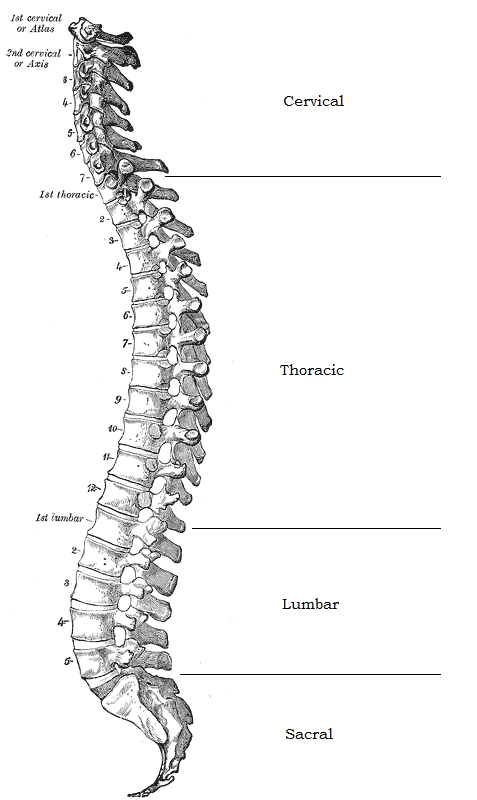
\includegraphics[width=7cm]{images/spine.png}
  \caption{Curvature of the vertebral column with the four regions labelled.
Adapted from \cite{Gray1918}.}
\label{fig:spine}
\end{figure}




The curvature of the spinal column features lordosis (concave curvature, when viewed from the posterior)
in the cervical and lumbar regions and kyphosis (convex curvature) in
the thoracic and sacro-coccygeal regions. It has been postulated that
the curvature exists to increase rotational stability -- moving mass
away from the centre line increases the centre of inertia about the
skull-pelvis axis. The change in curvature during gait cycle reduces the
loads on the skull due to absorption of energy in the tendons and
musculature of the surrounding areas. The curvature is created by
vertebral geometry in the thoracic and sacral regions, while in the
cervical and lumbar regions the curvature is created by the
intervertebral disc being wedge shaped.

\subsection{Vertebrae}\label{vertebrae}

Vertebrae vary greatly between each region and gradually within them.
Generally, vertebrae consist of the vertebral body on the anterior portion and the neural arch on the posterior portion along with pedicles and bony processes (Figure \ref{fig:vertebra}).

The vertebral body has a similar structure to long bones, with a
low-density trabecular structure internally, with a more dense cortical
shell. Due to approximately 80 percent of the compressive load of the
spine being carried by the vertebral body \cite{Adams2005}, the trabeculae are orientated
vertically to aid load transfer with horizontal trabeculae providing
resistance to compressive buckling. Especially in older patients, often
with osteoporosis, the vertebral body can be subject to vertebral
fracture, more commonly on the anterior portion, causing anterior collapse and a wedge shape when viewed from the side \cite{Adams2005}.

Vertebral bodies vary between level in terms of cross sectional area,
height and strength, with the axial strength of vertebrae increasing
from approximately 1300 N at the third cervical level to over 8000 N at the fourth lumbar level \cite{Stewart2006}. Similar variations have been found in the bone mineral density (BMD) \cite{yoganandan2006}, with the BMD varying
with the loads they are expected to carry. While a reduction in BMD is most often associated with osteoporosis, similar increases in the risk of fracture are attributed to metastatic bone disease.

\begin{figure}[hbt]
\centering

  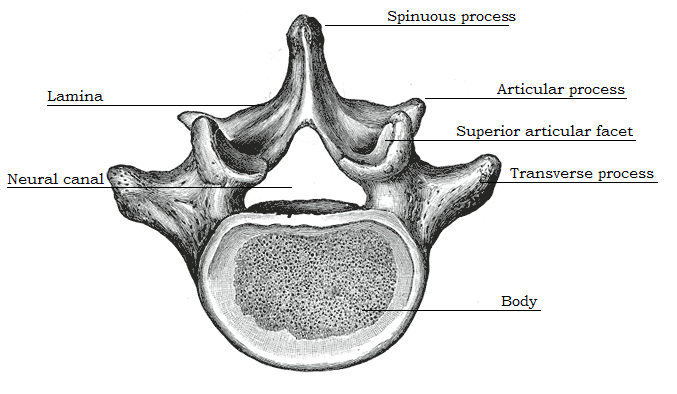
\includegraphics[width=10cm]{images/vertebra.png}
  \caption{Superior view of a lumbar vertebrae, with key features labelled.
Adapted from \cite{Gray1918}.}
\label{fig:vertebra}
\end{figure}


The posterior region of the vertebrae consists of two pedicles, followed
by the neural arch and processes. The spinous and transverse processes
allow for greater leveraging by the muscles and ligaments while the
superior and inferior articular facets of neighbouring vertebrae form
the facet (zygapophysial) joints.

Vertebrae at different levels have differing structures to permit their
required role. Cervical vertebrae are considerably smaller and lighter
than vertebrae at other levels due to the reduced weight they are
required to carry (the head and neck, and forces from stabilising
muscles). One identifying feature is the foramen transversarium lateral
to the vertebral body which allows for the passage of the vertebral
artery and vein \cite{panjabi1991cervical}.

The thoracic vertebrae vary substantially through T1 to T12 with the
size of the vertebral body gradually increasing and the pedicles
changing in orientation and shape. The addition of adjoining ribs
through the thoracic region greatly increase the stiffness of the
section due to the ligaments and costovertebral joints.

The lumbar vertebrae carry the greatest load of the spinal regions
\cite{Stewart2006} and consequently have the lowest height to width ratio
\cite{Manohar1992}.
The end-plates (at the top and bottom of a given vertebra) of this region are in general parallel, suggesting that
the lordosis originates from the disc shape rather than the vertebrae.

The sacral vertebrae are fused to form the sacrum which are followed by
three to four elements that form the coccyx and fuse in adulthood.
\section{Vertebral Fractures \&
Vertebroplasty}\label{vertebral-fractures-vertebroplasty}

\subsection{Vertebral Fracture Types}\label{vertebral-fracture-types}

The two most frequent types of vertebral fracture are the compression
fracture and the burst fracture. These types originate from different
conditions of both the intact vertebrae and the loads applied. To
examine the type of fracture, the vertebra is often categorised into
three columns from a sagittal view, with the columns being: the anterior
, middle and posterior regions \cite{Denis1983}.

\subsubsection{Compression Fractures}\label{compression-fractures}

A vertebral compression fracture (VCF) is a failure of the vertebral
body under the anterior column with the middle column remaining intact,
a feature unique to this type of fracture \cite{Denis1983}. Such fractures can
also be identified through compression of the cancellous bone and lack
of fragmentation. The two main types of VCF are anterior and lateral,
with the mechanism being anterior flexion and lateral flexion
respectively. These types can be further divided based on whether the
superior or inferior end-plate experienced failure, however failure of
the superior end-plate is more common \cite{Denis1983}. Radiographically, the
anterior
height of the vertebral body is reduced with no visible change or damage
to the posterior region of the vertebral body \cite{Denis1983}, although
occasionally in juvenile and osteoporotic vertebrae the damage is
limited to end-plate impaction \cite{Magerl1994}. A more extreme case
is a
vertebral body collapse, found in osteoporotic spines, where
occasionally fragments of bone are produced which can violate the spinal
canal especially when both end-plates are impacted (such cases are
treated as burst fractures) \cite{Magerl1994}.

\begin{figure}[hbt]
\centering
  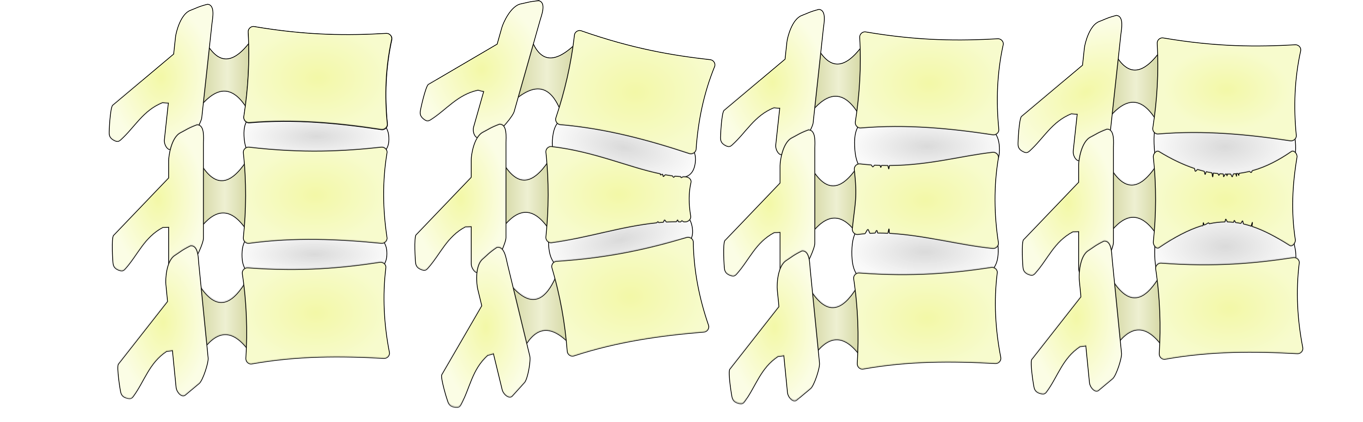
\includegraphics[width=\textwidth]{Chapters/Chapter_Lit_images/type_of_fracture}
  \caption{Types of VCF. Left: Intact FSU. Left-Mid: Anterior wedge fracture. Right-Mid: Posterior wedge fracture. Right: Vertebral body collapse. }
\end{figure}





A study of 132 anterior VCFs by Denis \cite{Denis1983} found that the
distribution of fractures favoured the upper lumbar region (L1 was
considerably more common) and mid-thoracic (T7 most common in the
thoracic region). Lateral VCFs accounted for only 16 of the 148 VCFs,
which were all found to occur in the lumbar region except one case.

\subsubsection{Demographic}

Patients suffering from vertebral compression fractures (VCFs) can
experience severe pain for extended amounts of time, dramatically
changing daily activities in addition to the pain, through reducing the lower vital capacity and forced expiratory volume when compared to patients without
such fractures \cite{Mathis2001}. Mortality rates were also reported to increase
with
VCFs in women, with the rate increasing further with the addition of
more fractures \cite{Mathis2001}.

Due to VCFs occurring most commonly through the loads applied to the
spine exceeding the axial strength of the vertebral body, the
demographic of sufferers is dominated by those with osteoporosis or
tumours within the vertebrae \cite{Mathis2001}. The occurrence of osteoporosis
is
usually age related with the frequency of VCF increasing from 25 percent
of postmenopausal women to 40 percent in women aged 80 years old in the
United States \cite{Studies2006}. However, as discussed by Melton \& Kallmes
\cite{MeltonIII2006}, there is difficulty in defining VCFs due to the number
of
systems developed to define them and the lack of a clear gold
standard for classification. This study found that the prevalence varied from 7\% to 19\%
for women in the age range of 50-80 years depending on the method by
which the fracture was defined and 4\% to 17\% for men in the same age
range. The prevalence of osteoporotic VCFs in women was found to be
twice that of men in an age-adjusted study \cite{Cooper1992}.

VCFs due to tumour infiltration into the vertebrae is another subset of
patients and was the motivation for the first image guided percutaneous
vertebroplasty procedure in 1984 \cite{Burstein1987}, however it is
difficult
to
assess the rate of such occurrences. The increasing ability to treat
osteolytic metastases and myeloma, leave more patients open to vertebral
collapse. This is further increased by possible secondary osteoporosis
induced by the treatment of malignant lesions \cite{Mathis2001}. However,
specific
pathologies and trauma account for a mere 3\% and 14\% respectively of
all clinically relevant fractures \cite{MeltonIII2006}.

\subsection{Risk Factors}\label{risk-factors}

Many of the risk factors of VCFs are the same as osteoporosis due to
their linked nature and can be categorised into potentially modifiable
and non-modifiable risk factors \cite{Studies2006}. Non-modifiable factors
include
age, gender, Caucasian race and history of existing fractures;
modifiable factors include insufficient physical activity, calcium and
vitamin D deficiency and alcohol and tobacco use \cite{Studies2006}.

\subsection{Diagnosis}\label{diagnosis}

Approximately two thirds of VCFs are undiagnosed \cite{Cooper1993} due to back
pain often being regarded as a consequence of aging and not reported by
patients. Care is often required to ensure that pain is directly related
to a VCF and not another spinal entity such as facet arthropathy,
herniated disc and spinal stenosis \cite{Mathis2001}. Indicators for Percutaneous Vertebroplasty (PVP) are
often
described as pain localised to the area, which lacks suggestions of
nerve or cord compression and includes an increase in pain under
weight bearing \cite{Mathis2001}. Vertebral pain for 1-6 weeks that fails to
reduce
after oral analgesics has also been defined as an indicator \cite{Diamond2006}.

Due to the strong relationship between BMD and bone strength, with
stronger vertebrae exhibiting a higher BMD \cite{Moro1995}, dual energy
X-ray
absorptiometry (DEXA) or quantitative CT can be used to predict
vertebral fractures. Increasingly the ability to assess the bone
structure at the clinical level gives a greater ability to clinicians to
predict fractures more accurately, due to BMD effectively being a
surrogate for the trabecular structure.

\subsection{Vertebroplasty}\label{vertebroplasty}

The main group of patients that receive
PVP are those with either osteoporotic VCFs or those with tumour
infiltration. Early use of PVP was limited to those patients who
responded poorly to conservative treatments, including analgesics, bed
rest, physical therapy and in some cases bracing \cite{Mathis2001}. However due
to
the low complication rate of PVP, indication of an osteoporotic VCF is
often enough and helps to reduce further compression of the vertebral
body \cite{Diamond2006}. PVP consists of the injection of bone cement into the
vertebral body from the posterior side of the body. The addition of
cement into an osteoporotic, fractured vertebral body allows
stabilisation of the fracture with the aim of reducing pain for the
patient.

\subsubsection{Vertebroplasty Procedure}\label{vertebroplasty-procedure}

Performing vertebroplasty requires careful monitoring during cement
injection and cannula placement; this is carried out with the use of
fluoroscopic guidance, which helps to limit the possibility of
extravasation (cement leakage from the vertebral body). Biplane fluoroscopy is often used, allowing the procedure
to be carried out more rapidly, while single plane fluoroscopy requires
checking both lateral and anteroposterior projections \cite{Mathis2001}.

There are three common approaches to the vertebral body: transpedicular,
parapedicular, and oblique, shown in Figure \ref{fig:vpapproach}.
Transpedicular
vertebroplasty
provides
a
route into the vertebral body through the pedicle, which acts as a
tunnel reducing the risk of dural puncture. Depending on patient
vertebrae size and level, the pedicle may be insufficient to allow
passage of the vertebroplasty needle and hence other approaches may be
required. The transpedicular approach also often requires injection from
both sides of the vertebrae into the vertebral body to prevent build-up
of cement on one side.

\begin{figure}[hbt]
\centering

  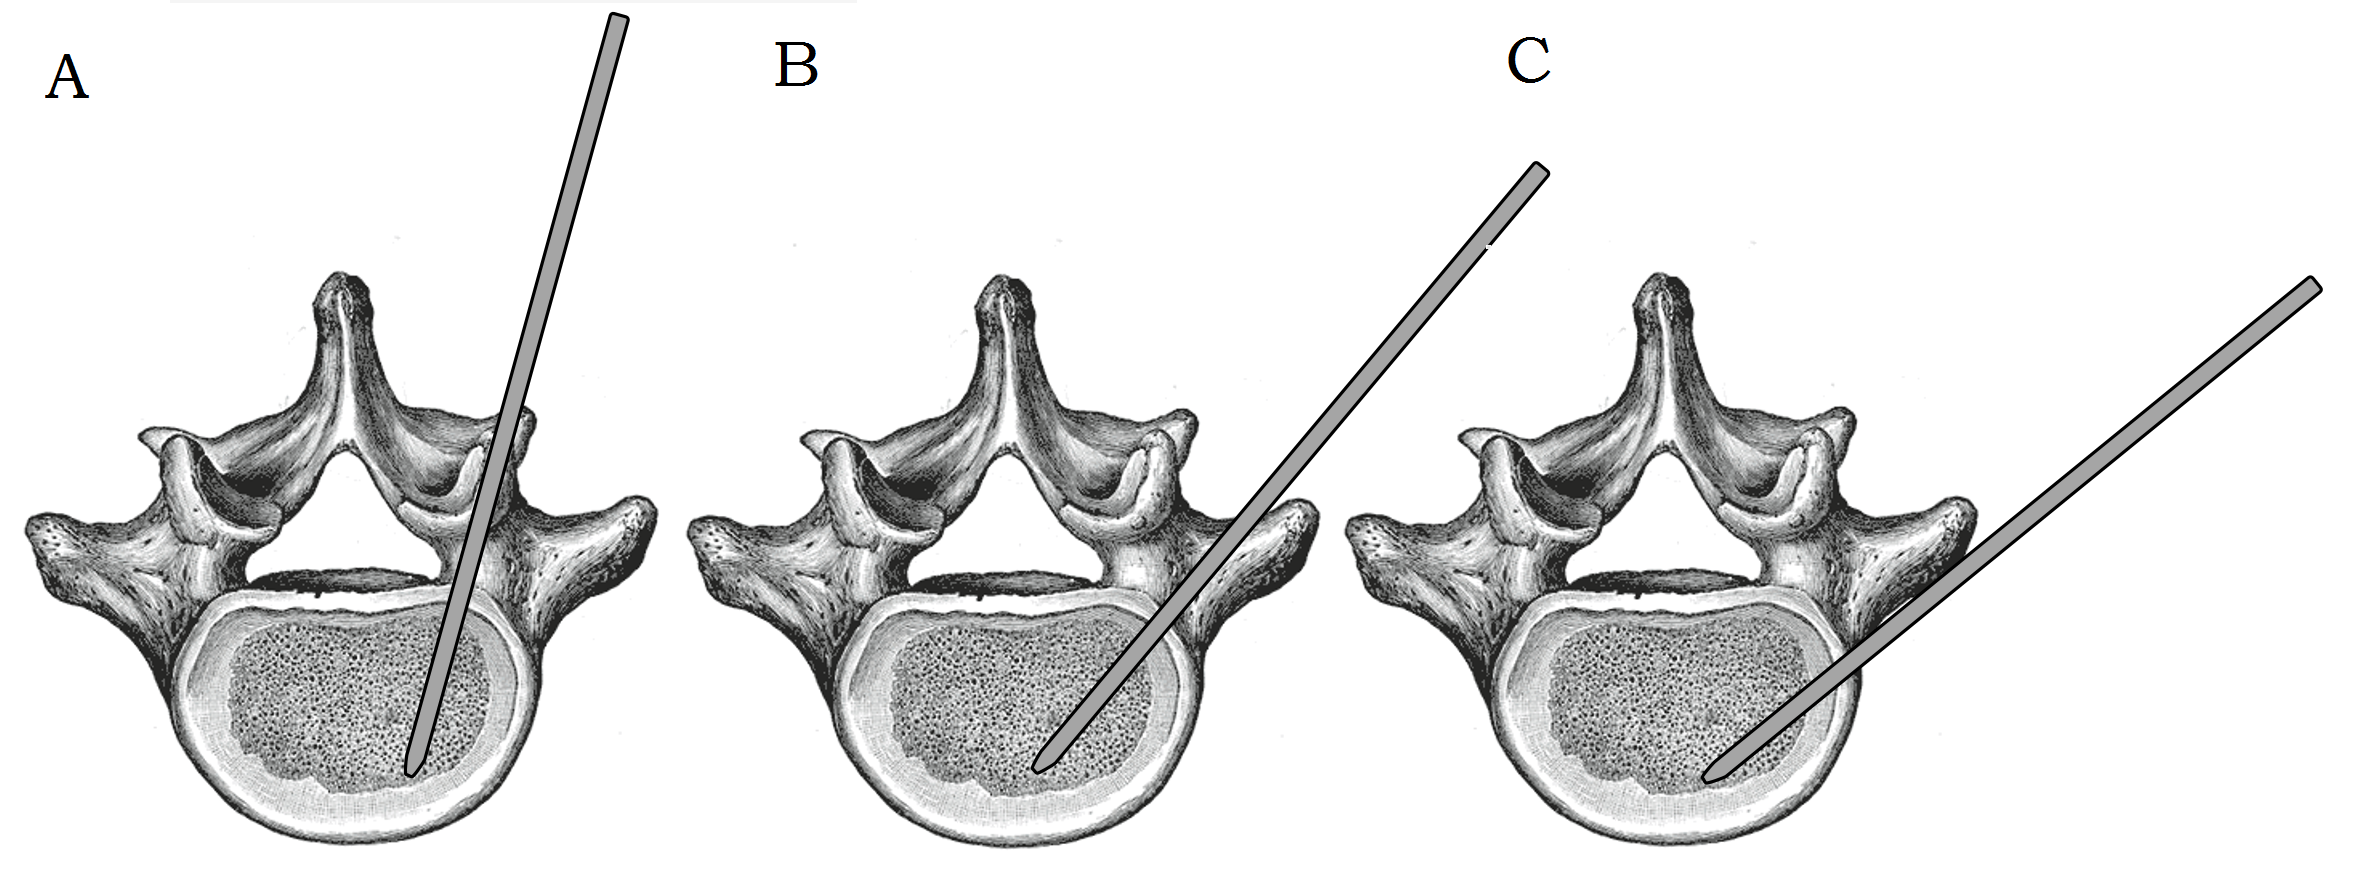
\includegraphics[width=14cm]{images/Vertebroplasty_approach.png}
  \caption{Three approaches to vertebroplasty. A, transpedicular approach, B,
parapedicular approach, C, oblique approach. Adapted from \cite{Gray1918}.}
\label{fig:vpapproach}
\end{figure}



The parapedicular approach involves the needle being inserted transversly across the pedicle until the
vertebral body wall is reached. It has the advantages of allowing the
needle to be positioned ideally for injection, removing the need for
multiple injections to evenly distribute the cement. Although allowing
ideal positioning of the needle tip, it requires the needle to pass
close to the basilar vein, therefore increasing risk of puncturing the
vein.

Finally, the oblique approach avoids the pedicle entirely, entering the
vertebral body in the posterolateral corner and is often used in the
thoracic region where the needle can pass over the top of the rib into
the vertebral body. Disadvantages of this approach include difficulties
in positioning due to the longer needle required and due to the
positioning any extravasation at the needle entry point will be around
the exiting nerve root \cite{pope2014musculoskeletal}.


\begin{table}[hbt]
    \caption{Two randomised clinical trials, with their similar inclusion and
exclusion criteria and results for the study.}
    \label{tab:randclinical}
\begin{tabular}{P{2cm}|P{2cm}|P{2cm}|P{2.5cm}|P{2.5cm}|P{2.3cm}}
Study Author & Number of patients & Type of pathologies & Inclusion Criteria & Exclusion Criteria & Results for osteoporotic patients\\ 
\hline
\hline
Buchbinder et al. \cite{Buchbinder2009} & 71 patients, 35 in VP group, 36 in
placebo group & Vertebral
compression fractures & Pain \textless{} 12 months
duration and presence of one or two vertebral fractures & \textgreater{}
90 \% collapse, presence of spinal cancer, retropulsion of fragments,
hip fracture or infection & No beneficial effect of vertebroplasty over
a sham procedure at 1 week or at 1, 3, or 6 months among
patients\\
\hline
Kallmes et al. \cite{Kallmes2009} & 131 patients, 68 VP group and 63 placebo
group
& Vertebral compression fractures & \textgreater{} 50 years of age 1--3
painful, osteoporotic vertebral compression fractures between vertebral
levels T4 and L5. Fracture \textless{} 1 year old & Evidence of
neoplasm, retropulsion of fragments, hip fracture or infection & No
significant difference between groups one month after the procedure on
measures of back pain intensity, functional disability, and quality of
life\tabularnewline

\end{tabular}
\end{table}

\subsubsection{Results of Vertebroplasty and Clinical
Trials}\label{results-of-vertebroplasty-and-clinical-trials}

The pain relief reported following vertebroplasty is currently not fully
understood; theories include effects on the nerve endings, both thermal
and/or chemical, and the general stabilisation of the vertebrae due to
the material properties of the cement which can restore the vertebral material properties
\cite{belkoff2001biomechanics}. The identification of factors that affect
pain relief are
often difficult to spot, especially with the relatively small patient
populations reported in studies, for example the study by Barr et al.
\cite{belkoff2002ex}, with 47 patients was able to find trends showing
patients with
single level fractures responded better to the procedure. However, the
importance of other factors such as degree of kyphosis and compression,
age, gender and fracture location require a much larger population in
order to obtain any statistical significance.

A large systematic review by Hulme et al. \cite{Hulme2006} of 69 clinical
studies achieved contrasting results to the study described above. A
large proportion of patients, 87 \%, had pain relief of some degree out
of 1552 patients from 32 studies. However, the review also found higher
than expected leakage rates, with leakage occurring in 41 \% of
vertebroplasty procedures and frequent new fractures were found above
and below the augmented level. These fractures give an example of the
need for larger, comparative, blinded and randomized clinical trials,
which could determine whether these fractures are a feature of altered
loading, increased patient activity or whether the new fractures would
have occurred regardless of the vertebral augmentation.

The two studies summarised in Table \ref{tab:randclinical} detail blinded
randomised and
controlled studies by Buchbinder et al. \cite{Buchbinder2009} and Kallmes et
al.
\cite{Kallmes2009}. These studies raised questions over the risks and evidence
for
vertebroplasty due to their conclusions that there is no difference
between the vertebroplasty and placebo groups. The near simultaneous
publication of such results caused many to disregard much of the
positive evidence \cite{Muijs2011} for vertebroplasty. However there are some
considerations regarding both of the trials: the inclusion and exclusion
criteria detailed in Table \ref{tab:randclinical} were neither clear nor well
defined,
failing to take results of MRI scans (Kallmes et al. \cite{Kallmes2009}) and
physical examinations (both) into consideration. Such results would link
to accepted indications of bone marrow oedema and pain on palpation
respectively \cite{Jay2013}. In addition to a population bias towards
fractures less than six weeks old, there was no statistical significance
between chronic and sub-chronic patients (due the small numbers),
prohibiting any insight into which subgroups of patients respond best to
vertebroplasty. Additionally, the National Institute For Health And Clinical Excellence guidance document suggests that consideration for receiving the treatment should be after six weeks, due to the severity of pain reducing over that time and many patients being pain free at six weeks post fracture \cite{Nice2013}. The standard deviation for both pain intensity and
Roland--Morris Disability Questionnaire scores were generally high,
especially at one month post-procedure. For example the mean ($\pm$SD) RDQ score in the vertebroplasty group was 12.0$\pm$6.3, as compared with 13.0$\pm$6.4 in the control group. This highlights the need to
understand where this variation originates from and hence which subset
of patients the treatment is better suited to.

\section{Experimental Studies}\label{experimental-studies}

\subsection{Trabecular Structure }\label{trabecular-structure}

The biomechanical properties of the vertebrae are known to rely heavily
on the trabecular structure, especially the compressive strength and
stiffness which relates to the failure behaviour and elastic behaviour
respectively. The compressive strength originates from the architecture
of the load-bearing trabeculae, which is characterised by thick
trabeculae columns or plates oriented vertically and held in place by
much thinner horizontal trabeculae. This internal structure changes with
age; the vertical plates are reduced to columns through bone remodelling
and horizontal supports are often removed \cite{atkinson1967variation},
\cite{parfitt1984age}.
Osteoporosis is often defined by a reduction in the Bone Mineral Density
(BMD) of 2.5 standard deviations below that of a young, healthy member
of the population of the same gender. However, reports of poor
correlations between the BMD and vertebral fracture rates suggest that a
measure of BMD is not sensitive enough to solely determine fracture
risks \cite{Aaron2000}, hence the trabecular architecture must be studied using
more sensitive and specialised tests.

Methods for studying the trabecular structure of the vertebral body
usually involve mechanical testing of the vertebrae, or trabecular bone
samples in conjunction with a study of the bone density. The trabecular
structure and bone architecture in general can be identified through
calculation of the ash density and comparisons of the trabecular
structure through histological and $\mu$CT examination. The following
measurable parameters are usually measured using $\mu$CT and/or histological
images of the trabecular bone: the bone volume fraction (BV/TV),
connectivity density (Conn.D), Structural Model Index (SMI), degree of
anisotropy (DA) and the trabecular separation, number and plate
thickness (Tb.Sp, Tb.N and Tb.Th respectively) and are discussed in
detail in the following papers by Hulme et al. \cite{hulme2007regional} and Mosekilde et al.
\cite{mosekilde1987biomechanical}.

The ash density allows comparison of the densities of bone samples
through the removal of water and soft tissue in addition to a
calculation of the mineral content using an additional measurement of
the dry weight. Bone marrow and other remaining soft tissue (fat) is
often removed prior to incineration using high-pressure water jets and
acetone washes \cite{keller1994predicting}. The dry weight is measured
following drying
using a recommended 100$^\circ$C furnace for an hour
\cite{keller1994predicting}
and
the dry
density (gcm$^{-3}$) is the weight divided by the specimen volume. To ash the
specimens, they are usually placed in a muffle furnace at 650$^\circ$C for
18-24
hours\cite{mosekilde1987biomechanical}, \cite{keller1994predicting}, which
following cooling can
be reweighed. The
mineral content can be calculated through dividing the ash weight by the
dry weight and ash density by dividing the ash weight by the initial
specimen volume. However, with the adoption of $\mu$CT in most studies
regarding trabecular structure, ash density calculations are rarely
used in more recent studies.

Other parameters of bone architecture (BV/TV, Conn.D, SMI, DA, Tb.Th,
Tb.N and Tb.Sp) are usually defined through $\mu$CT scans of the bone and
analysis using accompanying software to the $\mu$CT scanner. The bone volume fraction, BV/TV, usually
quoted as a ratio or percentage, is a measurement of the proportion of
the total volume of interest that is bone tissue. Conn.D indicates the
number of trabecular connections per volume of interest. The SMI
provides a quantification of numbers of different types of trabecular
element, usually on a scale from 0 to 3 (from rods to parallel
plates)\cite{hildebrand1997quantification}. Tb.Sp and Tb.Th are measured in
length and identify the
average separation between trabeculae and the thickness of trabeculae
respectively, while Tb.N quantifies the number of trabeculae per unit
length. Finally, the degree of anisotropy measures the average alignment
of the trabeculae along a specific axis, where a value of one usually
specifies isotropic behaviour and less than one equates to various
degrees of anisotropy\cite{hulme2007regional}.

The region of interest for taking specimens from the vertebral body
depends on the nature of the study. If the study requires the capture of an
average value for the vertebrae, then the largest possible
volume of cancellous bone is required, while avoiding the cortical bone
and areas where the basivertebral vein intersects
\cite{yoganandan2006}.
Other
studies
have included all cancellous bone between the cranial and caudal
endplates and have used subsections of the vertebral body to identify
differences and changes with age to specific regions \cite{hulme2007regional}.

Bone morphology has been shown to vary greatly between different regions
of the vertebrae \cite{hulme2007regional}, \cite{thomsen2002zone} and between
different ages
of
vertebrae \cite{thomsen2002zone}, \cite{ebbesen1999age}. Animal models are
commonly used for
the in
vitro and in vivo biomechanical models of the spine while testing the
performance of various treatments. However, despite providing a basic
understanding of spinal function, the differences in vertebrae at
different levels and the changes that the vertebrae experience with ageing
mean a single species cannot be used to model the entire spine. Hence
many different large mammals have been used, including bovine, ovine,
porcine and cervine vertebrae which have already been characterised in
the literature \cite{wilke1997sheep,kandziora2001comparison,kumar2000anatomy}. These studies
compare the
anatomical
variation in terms of vertebral body width, height and depth, spinal
canal size and pedicle height and width. Studies detailing similar
anatomical properties for human vertebrae also exist, allowing
comparison and assessment of whether a particular animal model is
appropriate \cite{panjabi1991cervical,Manohar1992}. The
anatomical differences found
between
the animal study papers listed above and the human studies show many
differences between all of the parameters, furthering the idea of
multiple animals being used for different studies. The studies suggested
that sheep spines were much larger than humans, with the vertebral body
height being particularly greater \cite{kumar2000anatomy,kandziora2001comparison}, while the
mean
vertebral width and depth of the human spine are greater than that of
all the animals in the studies (with the exception of the upper thoracic
segments in the deer \cite{kumar2000anatomy}). Much of the geometric and structural variation between human and animal vertebrae may be due to the orientation during walking and therefore load differences. Despite this large difference, muscle forces may add additional loads to the vertebrae, reducing the total loading differences.

A study regarding the trabecular composition of bone samples from the
lumbar spine compared: human, dog, pig, cow and sheep and concluded that
care was required when choosing a suitable animal model for a particular
study, due to the large interspecies differences in terms of Bone Mineral Content (BMC),
volumetric BMD (vBMD), height and area and finally fracture stress
\cite{aerssens1998interspecies}. They found that human BMC and vBMD were
significantly lower
when compared to the other animals in the study, aligning with the
greatly reduced fracture stress also reported; the details of this can
be seen in Figure \ref{fig:bmdgraph}. However, the study also reports a
higher fracture
stress in sheep compared to cows, yet similar values for the BMC and
vBMD, with a similar trend also found between pigs (higher BMD) and dogs
(lower BMD). Having similar density properties yet high fracture stress,
aligns with reports of poor correlations between the BMD and vertebral
fracture in the study by Hordon et al\cite{Aaron2000}.



\begin{figure}[hbt]

\centering
  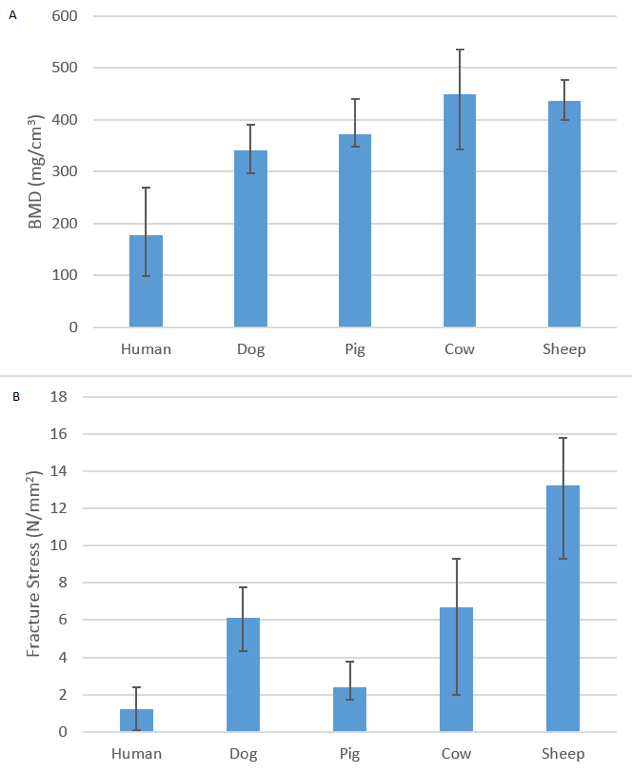
\includegraphics[width=4.21209in,height=5.15601in]{images/bmdGraph.png}
  \caption{A, the mean BMD from
cylindrical cores taken from the lumbar spine of five different species.
B, the mean fracture stress for the same five samples. Bars indicate the
range of values. Adapted from \cite{aerssens1998interspecies}.}
\label{fig:bmdgraph}
\end{figure}

\subsection{Current Studies on Vertebral Fractures and Vertebroplasty
}\label{current-studies-on-vertebral-fractures-and-vertebroplasty}

There have been a considerable number of experimental studies that have investigated the
effects of vertebroplasty through mechanical testing. Often
these studies are carried out in conjunction with computational studies,
where properties are defined experimentally and used to validate
computational models, for example \cite{Wijayathunga2008}. These studies are reviewed in the following section, with a focus on the preparation of
specimens and
methods and with references to notable findings.

\subsubsection{Specimen Preparation }\label{specimen-preparation}

Capturing as much data as possible for a given specimen is vital for understanding
results and allowing those results to be used in many areas of study.
Hence, pre and post-mechanical loading $\mu$CT scans (including
scans before and after cement augmentation) are usually captured.

To simulate physiologic conditions, specimens are often wrapped in
phosphate-buffered-solution (PBS, saline) soaked gauze following
dissection \cite{belkoff2002ex} and are stored at -20$^\circ$C and
thawed for 24
hourssubsubsection
before testing at a non-physiological room temperature\cite{tarsuslugil2013development},
\cite{furtado2007biomechanical}. This difference between room and body temperature may affect the results, whith constituents of the specimens, such as the bone marrow, having different properties at the two temperatures. However, there is a lack of research investigating the effects temperature has on mechanically testing specimens in the literature.


\subsubsection{Mechanical Testing }\label{mechanical-testing}

The generation of vertebral fractures experimentally attempts to match the natural
creation of such fractures; compression fractures are usually generated
with an application of force at a low rate, mimicking the gradual creation of fractures in osteoporotic vertebrae
over time. Natural burst fractures are
usually the result of a traumatic event, high energy impacts causing high
rate axial loads through the vertebrae; experimentally burst fractures
are usually generated through dropping a load of known mass onto the
specimen from a calculated height \cite{tarsuslugil2013development},
\cite{wilcox2004dynamic},
generating
comparative forces to a natural traumatic impact. However, other methods
involving biaxial hydraulic testing machines, where high loads (50 --
100 \% of the animals body weight) were applied over a short period of
time, generating the burst fracture \cite{Gurwitz1993}.

Mounting of specimens prior to loading in material testing machines
allows the position of vertebrae to be maintained during testing, whilst
not restricting or confining compression more than necessary. Methods of
mounting allow parallel positioning of the exterior surfaces and allow
perpendicular loading of the vertebrae along the axis. These
requirements for the mounting are usually achieved through potting the
specimens in PMMA \cite{tarsuslugil2013development, furtado2007biomechanical, ananthakrishnan2005effect}, semi
cured moulding
material \cite{berlemann2002adjacent} or low viscosity resin
\cite{pneumaticos2013effect}.

Methods of loading both a pre-fracture and post fracture/augmentation
rely on mimicking the natural loading of the spine, with similar methods
being used throughout the literature. Loading is carried out with a
materials testing machine, applying loads either under pure axial
compression or allowing flexion of the upper endplate through various
methods. Methods of applying the ``natural'' load include applying the
load or displacement through a steel ball, requiring a specified loading
point and allowing natural motion \cite{tarsuslugil2013development},
\cite{furtado2007biomechanical}.
Applying bilateral
loads through pneumatic cylinders and allowing controlled flexion with
simultaneous compression \cite{ananthakrishnan2005effect} and similarly with
the application of
two anterior and two posterior loads using pneumatic cylinders
positioned so that more of the load was applied to the anterior side
causing flexion \cite{pneumaticos2013effect} were other methods used in the
literature.
The positioning of the applied load differs in the literature varying
between the mid point of the superior endplate \cite{Barr2000} and one quarter
of the distance of the vertebral body in from the anterior margin of the
superior endplate \cite{belkoff2001biomechanics}. With some studies identifying the effect of loading position on the measured stiffness of the vertebrae \cite{Wijayathunga2008}.

The definition of the point of fracture varies in the literature, most
commonly the fracture point was defined as the peak on the recorded
load-displacement graph. However, Furtado et al. \cite{furtado2007biomechanical} defined the point of
fracture creation as 75\% of the original vertebral body height, with
the failure strength defined as either the value at the end of the
experiment (75\% of VB height) or the peak on the load-displacement
graph. Pneumaticos et al. \cite{pneumaticos2013effect} defined the point of
fracture (or
maximum fracture load) using the load-displacement graph, where
catastrophic failure could be observed through a sudden jump in the
displacement.

\subsubsection{Results of Mechanical Loading
}\label{results-of-mechanical-loading}

Mechanically loading vertebrae in the study by Furtado et al. \cite{furtado2007biomechanical} showed a
significant correlation between failure strength and the product of BMD
and endplate area, with the range of failure loads being 900 N to 2200 N
for human thoracic vertebrae between T2 and T12. However, the failure
load was defined as the load at a deformation of 75 percent of the
original vertebral height or the peak load before reaching this
deformation, potentially suggesting that the maximum load was not
achieved until after 25 percent strain. This may explain the discrepancy
between these results and those of Pneumaticos et al.
\cite{pneumaticos2013effect} where the
average reported failure load was 6724 $\pm$ 3291 N for intact specimens
using vertebrae between the thoracic levels T2 to T11 from four human
cadaveric spines.

\subsubsection{Experimental Vertebroplasty Compared with Clinical
Vertebroplasty
}\label{experimental-vertebroplasty-compared-with-clinical-vertebroplasty}

Experimentally, transpedicular (uni or bi-pedicular) approaches are more
common in the literature\cite{furtado2007biomechanical, ananthakrishnan2005effect, pneumaticos2013effect},
although
extrapedicular approaches have also been used \cite{furtado2007biomechanical}.

Although bilateral transpedicular vertebroplasty is the more common clinical
procedure\cite{tohmeh1999biomechanical}, unipedicular vertebroplasty is used
under some
mitigating circumstances often requiring the patient to return for the
second injection. A study comparing bilateral and unilateral
vertebroplasty found no significant difference between the two
procedures in terms of vertebral height and stiffness, possibly
attributed to the central positioning of the cement despite the
unilateral approach \cite{tohmeh1999biomechanical}. The authors reached the
conclusion that a
unipedicular approach is a valid alternative to bipedicular
vertebroplasty and may be especially useful during multilevel
vertebroplasty by reducing the number of injections and hence risk of
cement leaking outside the vertebral walls (extravasation).

\subsubsection{Results following Experimental Vertebroplasty
}\label{results-following-vertebroplasty}

\begin{landscape}

\begin{table}[h]
\caption{Comparison of the
methods used in studies carrying out vertebroplasty experimentally on
cadaveric specimens.}
\label{tab:vpmethods}
\begin{tabular}{P{2.5cm}|P{5cm}|P{5cm}|P{5cm}|P{5cm}}
Author & Type of specimen & Procedure type \& fill volume & Cement Type
& Key Finding\\
\hline
\hline
Belkoff et al. \cite{belkoff2000biomechanical} & Five vertebral bodies (L1--L5)
from four female cadaveric spines (age, 80 $\pm$ 5 years) &
Transpedicular, 6 ml
fill volume throughout & A bioactive cement, Orthocomp (Orthovita, Malvern,
PA) \& a PMMA based cement, Simplex P (Howmedica, Rutherford, NJ) &
Significantly greater strength following injection of cement, compared
to the intact vertebrae \\
\hline
Furtado et al. \cite{furtado2007biomechanical} & Twenty-six single vertebrae
from 2 female
cadavers (age, 88 and 89 years) & Extrapedicular into anterior third of
vertebral body, 20 \% volume fill, based on height x endplate surface
area & PMMA with 20 \% by dry weight of barium sulfate & Increased
failure strength by a factor of 1.72 post vertebroplasty compared to the
intact vertebrae \\
\hline
Higgins et al. \cite{Higgins2007a} & Human cadaveric, 61 vertebrae from 5
cadavers
with mean age of 81 years & Unipedicular, 10\% and 20\% cement fill by
volume, with unfilled as controls & PMMA & A statistically significant
36\% strength increase as compared with the unfilled controls regardless
of density levels \\
\hline
Pneumaticos et al. \cite{pneumaticos2013effect} & 40 vertebrae from four human
cadaveric
thoracic spines (age range 65-69 years) & Transpedicular, 6 ml fill
volume throughout & PMMA, with 5 to 1 ration of barium sulphate & A
reduced failure load post vertebroplasty, although
non-significant \\

\end{tabular}
\end{table}

\end{landscape}

The methods used to recreate the vertebroplasty procedure experimentally
vary considerably between studies, especially given the sensitivity that
certain studies suggest factors such as fill volume have on outcomes.
Table \ref{tab:vpmethods} shows the methods and some of the more important
variables used
in a selection of studies carrying out vertebroplasty on cadaveric
specimens. Below is discussion of some of the finer points of the
studies, including comparisons to clinical studies.

Identifying the effect of vertebroplasty on intact specimens in the
thoracolumbar region, Higgins et al. \cite{Higgins2007a} found the strength was
increased by a statistically significant amount of $\sim$36\% using 20\% fill volume
and that when comparing the strength increases with BMD, it was found
that those vertebrae with a lower BMD showed a more dramatic increase in
the strength. Conversely Graham et al. \cite{Graham2003}, found that highly osteoporotic
vertebrae showed the least improvement compared to intact vertebrae in
terms of strength and stiffness. 

Higgins found that the upper thoracic
vertebrae failed to show any significant result following augmentation
of both 10 \% and 20 \% compared to the intact controls. Belkoff et al.
\cite{belkoff2000vertebroplasty} suggested that 7.7 mL of cement was required
to restore the
original strength of fractured osteoporotic vertebrae, this corresponded
to $\sim$24 \% volume fill in the lumbar vertebrae tested. 

When comparing different cements Belkoff
\cite{belkoff2000biomechanical} found that in order to obtain a significant
increase in the
strength 6 mL or approximately a fill of 18 \% was required. Similarly,
Lee et al. \cite{lee2002prediction}, found that between 25 \% and 30 \% volume
fill was
required to restore strength to the intact level for lower thoracic and
lumbar vertebrae in a clinical study. Graham et al. \cite{Graham2003}, required a fill
volume of 24 \% (average 7 mL) to achieve statistical significance,
however this did not return the stiffness to the intact level, and only
returned the strength to the intact level in those specimens with the
highest BMD of their group.

An increase in strength following fracture and augmentation is a
desirable outcome especially for osteoporotic vertebrae where
returning the strength to that of the intact vertebrae may not prevent
fractures. This is often carried out as prophylactic percutaneous vertebroplasty, where the procedure is carried out on vertebrae that are likely to fracture or on levels adjacent to fractured vertebrae already undergoing PVP. Restoring the stiffness however is believed to be responsible
for pain relief due to the internal stabilisation and prevention of
micro motion, providing a more suitable environment for healing. A study
examining the quantity of cement required to restore the strength and
stiffness of osteoporotic vertebrae having undergone a compression
fracture found that as little as 2 mL of cement is enough to restore the
strength of the vertebrae to the intact value, with the quantity
required to restore the stiffness being between 4 mL and 6 mL depending
on the level (lumbar vertebrae requiring more
cement)\cite{belkoff2001biomechanics}.

Regarding extravasated cement during the vertebroplasty procedure,
Higgins et al. \cite{Higgins2007a} found that an increase in the BMD greatly
increased the tendency for cement to leak, however, this typically was from
the anterior wall of the vertebra (more favourable than into the spinal canal) and was independent of vertebral
level.

Despite previous studies suggesting BMD alone could not be used as an
indicator for vertebral fracture \cite{Aaron2000}, Higgins et al. concluded
that
it was one of the most important factors, conceding however that the BMD
measured ex-vivo is not directly comparable to that measured in a
clinical setting. This was due to differences in the BMD calculation due to the surrounding soft tissue for the \textit{in vivo} scans.

The results from Furtado et al. \cite{furtado2007biomechanical} using an
extrapedicular
vertebroplasty approach achieved approximately 25 \% fill for specimens
which had previously undergone loading to generate a compression
fracture, equating to an average volume of cement of approximately 4.5 ml.
This
augmentation caused a significant increase in the failure load, a factor
of 1.72 increasing the average failure load from 1.61 kN $\pm$ 0.49 kN to
2.63 kN $\pm$ 0.85 kN. A similar result was achieved by Tohmeh et al.
\cite{tohmeh1999biomechanical}, showing that the post augmentation strength is
significantly
higher than the fractured and intact vertebrae. Pneumaticos et al.
\cite{pneumaticos2013effect} found no significant difference between intact and
post
augmentation intact vertebrae, with an average failure load of 5.77 $\pm$
2.13 kN for the augmented intact specimens with 6 mL of cement
injected.

% TODO Discussion of Experimental Studies
%\subsection{Discussion of Experimental Studies}
%
%The results presented above describe a wide ranges of approaches to measuring vertebral variables. The range of 

\section{Finite Element Modelling
(FE)}\label{finite-element-modelling-fe}

The use of finite element models of the spine, spinal segments and
vertebrae has been rising rapidly over the past decades. They are being
used to model a range of interventions and devices along with being used
to aid our understanding of spinal biomechanics. The main benefit of
such studies is the ability to test a range of variables and properties
for the same model or specimen, with an additional benefit of assessing
parameters that cannot easily be measured experimentally, such as stress and
strain fields.

Important factors for the generation of biomechanical finite element
models have been discussed previously \cite{Jones2008}--\cite{Viceconti2005}
and include
verification, sensitivity testing and validation of models created. The
first of these factors is an assessment of the numerical accuracy of
the model; given that most studies use commercially available software
for FEA this verification has usually already been carried out, with
documentation available. Additional verification can be carried out
regarding mesh sensitivity and convergence, where the level of detail of
the model is investigated with considerations of accuracy and
computational cost. Sensitivity testing determines the sensitivity of a
model to various input variables and the errors that these input
variables have on the system. Such tests may include the response of the
system to various boundary conditions and material properties.
Validation of models is a proof that the computational results agree
with either \emph{in vitro} or \emph{in vivo} results, however, proof
that the results agree with the \emph{in vitro} model do not mean that
the model is a valid representation of the \emph{in vivo} scenario.

Due to the importance of trabecular bone in many aspects of bone and
spinal research, the methods used to model it are quite detailed
throughout the literature. There are currently two dominant approaches
to modelling trabecular bone using FEA, discussed in detail by Mengoni
et al. \cite{Mengoni2014}. These are $\mu$-FE, which expresses the micro
structure
of
the bone explicitly, and continuum level FE models which represent the
trabecular structure through a continuous model using an inhomogeneous
material property to represent the micro-structure. The
increased computational cost of $\mu$-FE models, especially for full sized
vertebrae and larger functional spinal units, means that many studies use
continuum level FEA, despite the reduced level of
detail. However, the development of continuum level models allows the use of much larger CT scan data sets, given that the resolution of clinical $\mu$CT scanners is upwards of 1.2 mm$^3$.

The studies summarised in Table \ref{tab:geoNmesh} use various methods to
acquire
vertebrae geometry, generate models and apply appropriate material
properties, either from combinations of scan data and experimental data,
or homogenous experimentally defined properties. The variations between
methods and results which can be drawn from these studies is described
below.

\subsection{Geometry \& Meshing}\label{geometry-meshing}

With the growing availability of $\mu$CT scanners and the increasing
resolution available with them, studies using \emph{in vitro}
measurements and handcrafted geometries such as the study by Higgins et
al. \cite{Higgins2007a} in 2007 are being replaced with geometries developed
from
$\mu$CT data. One of the more common methods of generating specimen specific
models of vertebrae is the conversion of voxels from down-sampled $\mu$CT
images into hexahedral elements. The direct conversion of voxels into
elements has the advantage of increasing the simplicity of model
generation, however, this requires real specimens (in the form of animal or human tissue)
which can be difficult to acquire and scan.

\begin{landscape}

\begin{longtable}{P{0.2\textheight}|P{0.2\textheight}|P{0.7\textheight}|P{0.5\textheight}}
\caption{The geometry generation, meshing and material property
assignment methods for 7 studies modelling single vertebrae to acquire
stiffness and strength data.}
\label{tab:geoNmesh}
\\
Author & Geometry Generation & Meshing & Material Properties \\
\hline
\hline
Brown et al. (2014) \cite{RobsonBrown2014} & Used $\mu$CT with resolution of 0.074 x
0.074 x 0.074 mm & Using ScanIP software, segmented CT images down sampled to 1
x 1 x 1 mm and meshed in ScanFE using hexahedral elements and
tetrahedral elements for the smooth vertebral surface & Material
properties assigned using density values from $\mu$CT. No division between
cortical and cancellous bone. Relationship between elastic modulus and
BV/TV value investigated\\
 \hline
 Buckley et al. (2006) \cite{Buckley2006} & Used $\mu$CT data with resolution of 1 x 1
$\times$
1 mm &
Conversion of voxels to hexahedral elements of size 1 x 1 x 1 mm &
Material properties assigned using density values from $\mu$CT. No division
between cortical and cancellous bone\\
\hline
Chevalier et al. (2009) \cite{Chevalier2009} & Used HR-pQCT data with resolution of
0.082 x
0.082 x 0.082 mm & Used $\mu$CT data to find cortical wall thickness.
Surface meshes defined through local triangulation for each cell for the
surface and interior cortical wall boundary. Trabecular bone modelled
with hexahedrons of size 1.312 x 1.312 x 1.312 mm using GMSH software &
Elastic and yield properties assigned to each trabecular element from
$\mu$CT density data\\
\hline
Eswaren et al. (2007) \cite{Eswaran2007} & Used $\mu$CT data with resolution of 0.03 x
0.03 x
0.03 mm & Conversion of voxels to hexahedral elements of size 0.06 x
0.06 x 0.06 mm. 8 node hexahedral elements using in-house software.
Endplates and cortical shell modelled with higher definition using
thickness from $\mu$CT Bone within 180 $\mu$m of the outer structure was
identified as belonging to the cortical shell. & Used a constant
material property for entire model\\
\hline
Higgins et al. (2007) \cite{Higgins2007a} & Taken from in vitro measurements of L1
vertebrae, using flat endplates and curved side walls & Composed of 12
node brick elements using in-house code. Used separate mesh for cortical
walls and different thicknesses for the endplates and posterior and
anterior cortical shell. & Anisotropic through model, using different
material properties for cortical shell, endplates and vertebral
body.\\
\hline
Kinzl et al. (2012) \cite{Kinzl2012} & Used $\mu$CT with resolution of 0.082 x 0.082 x
0.082 mm & Used $\mu$CT data to find cortical wall thickness. Surface meshes
defined through local triangulation for each cell for the outer and
interior cortical wall boundary, meshed using pentahedrals. Trabecular
bone modelled with tetrahedrals & Material Mapping based on porosity
(density). Uses parameters for elastic, plastic and damage behaviour.
Uses elasto-plastic material for the cement augmented
region\\
\hline
Wijayathunga et al. (2008) \cite{Wijayathunga2008} & Taken from $\mu$CT data with
resolution 0.074
x 0.074 x 0.074 mm & Hexahedral and tetrahedral elements using ScanFE
software, smoothing is applied to vertebral surface to improve geometry
& Material properties assigned using density values from $\mu$CT. No
division between cortical and cancellous bone\\


\end{longtable}

\end{landscape}

The cortical surfaces of these models are often rough when just using
voxel to element meshing, for example the models created by Buckley et
al. \cite{Buckley2006} in Figure \ref{fig:buckleymesh}. However, many
studies
introduce
smoothing
to
the surface of a vertebra model. The error introduced from possible
stress raisers when omitting smoothing from the model was questioned by
Chevalier et al. \cite{Chevalier2009}. This study suggested that smoothing, in
the
form of surface meshes representing the cortical walls, successfully
removed the stress raisers and artificial damage zones from their
models. The studies by the group that produced the Chevalier et al. and
Kinzl et al. papers in Table \ref{tab:geoNmesh} use methods for fitting
the vertebrae
surface of the model to that of the scanned specimen, rather than simply
smoothing the voxel to element mesh. Kinzl et al. \cite{Kinzl2012} used a
``marching tetrahedral'' method to extract the surface of the scanned
vertebrae from Treece et al. \cite{Treece1999}, which uses an adaption of the
popular marching cubes method to obtain an iso-surface from discretised
three-dimensional data (from $\mu$CT data).

\begin{figure}[ht!]

\centering
  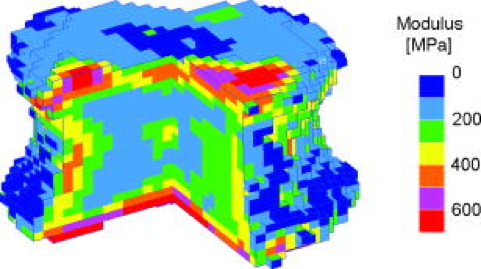
\includegraphics[width=3.20764in,height=1.79236in]{images/voxelFEMesh.png}
  \caption{Voxel finite element mesh of L2 vertebrae used by Buckley et
al. with voxel size of 2 mm \cite{Buckley2006}.}
\label{fig:buckleymesh}
\end{figure}


There is a reduced difference between the structure of the cortical shell and the
cancellous bone structure of the vertebra when compared to other human
bones \cite{Eswaran2005}. Despite this, the cortical walls have been shown to
share a significant quantity of the load, especially in the axial
midsection, where the cross section is narrowest and the load carried by
the cortical wall is greatest \cite{Eswaran2005}. An understanding and correct
modelling of the load sharing between the cortical wall and trabecular
bone becomes more important when considering the variation of the
cortical wall with age, location, level and osteoporotic nature of the
vertebrae in question \cite{Ritzel1997}. Chevalier et al. \cite{Chevalier2009}
found
that
adding a surface faced cortical shell to their models unloaded the
centre trabecular bone and increased the strength and stiffness values
of their models to that of their experimental results. Approaches that
rely on the $\mu$CT greyscale values to assign material properties to
elements, give additional stiffness to the cortical walls due to the
denser and therefore brighter cortical regions in the $\mu$CT images,
without the need for modelling the regions separately.

The increased resolution of the Eswaran et al. \cite{Eswaran2007} study allowed
for a uniform element size and material assignment for the cortical
shell and trabecular bone, relying on the resolution to represent the
higher density of bone within this region. In this case, separate meshes
were used for the two bone types (cortical and trabecular) to extract
information about load sharing between them. However, the required use
of a supercomputer to analyse the FE models limits such models being
used within research, especially where large datasets are required to
investigate population variation.

\subsection{Material Properties}\label{material-properties}

Material properties for continuum level FE models are in general derived
from BV/TV values from $\mu$CT greyscale data for each voxel and assigned to
the matching element. These density values are used to derive elastic
modulus values using a conversion equation. This conversion equation is often optimised to choose the best values for the conversion equations such the the error between experimental and computational results are minimised. Robson Brown et al.
\cite{RobsonBrown2014}
performed an investigation into the effect of a linear or non-linear
relationship between the elastic modulus and BV/TV. However, due to
lower order errors in the form of the tissue modulus and degree of anisotropy, no benefit
was found when using the higher order relationship. A good
agreement was found with the linear relationship in the Robson Brown
et al study when using a similar method in the study by Wijayathunga et
al.\cite{Wijayathunga2008}.

Chevalier et al. \cite{Chevalier2009} and Kinzl et al. \cite{Kinzl2012} used
other
methods
of representing the material properties. In these studies an enhanced
continuum FE model was used where, rather than using the more common
method of converting $\mu$CT voxels directly into hexahedral elements, they
used high-resolution CT images, which included the cortex and used
fabric-elasticity relationships to describe bone morphology. This
deviation away from the more common methods used by others
\cite{RobsonBrown2014, Wijayathunga2008}, potentially allows $\mu$CT at lower resolutions to be
used, which
both reduces computational cost and introduces possibilities for the use
of clinically relevant resolutions. The use of lower resolutions was achieved by using 82 $\mu$m scans and coarsening them to 1.312 mm to mimic common clinical CT
scans. With a focus on identifying modelling errors, a study by Pahr and
Zysset \cite{Pahr2009} compared this enhanced continuum FE models with
standard methods. This study looked at both the effect of smooth cortex
modelling (also used by Chevalier and Kinzl) and the
morphology-elasticity relationship. Pahr and Zysset concluded that this
method of modelling provided statistically equivalent results for the
stiffness of two different models when compared to the more common
method, whilst analysing the model at least 100 times faster.
This reduction in time to analyse the models was due to the reduced sensitivity to mesh size, meaning
mesh density and therefore number of nodes / elements could be reduced.

\subsection{Modelling Vertebroplasty}

The methods used to model vertebroplasty from a selection of studies are
summarised in Table \ref{tab:modVP}. The variation in geometry
generation can be seen
to vary similarly to studies modelling vertebrae alone, however, in
addition to this, the generation of cement geometry and material
properties is also presented due to the range of methods used.

\begin{figure}[ht!]

\centering
  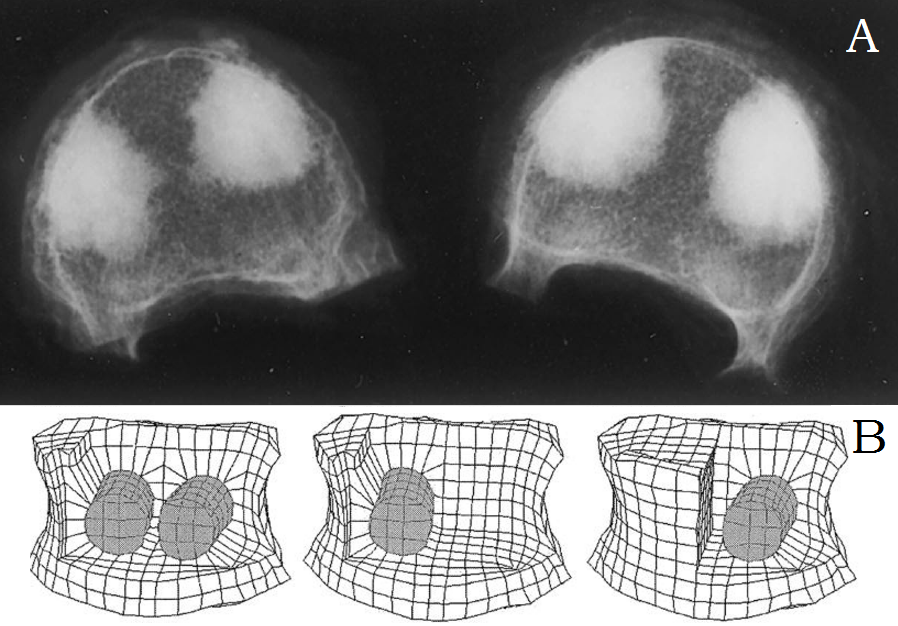
\includegraphics[width=4in]{images/VP_scan_vs_model_lit_rev.png}
  \caption{A: Top view $\mu$CT scans of human vertebrae augmented \textit{in vitro}, showing gradual reduction of cement opacity to the edges of the internal cement volume, adapted from Belkoff et al. \cite{belkoff2001biomechanics}. B: The augmented model generation for the study carried out by Liebschner et al. \cite{Liebschner2001}.}
\label{fig:VP_scan_vs_model_lit_rev}
\end{figure}

Methods of modelling vertebroplasty usually involve using $\mu$CT scans of
augmented vertebrae, masking the internal volume of cement though
thresholding the greyscale background. However, the methods used in the
studies by Liebschner et al., Polikeit et al. and Baroud et al.
\cite{Liebschner2001,Baroud2003,Polikeit2003} used approximations of the cement
distribution,
with
the former modelling the distribution according to images from \emph{in
vitro} experiments and clinical trial CT scans, while the other studies
modelled the cement more approximately. Such approximations of the internal volume of cement can be seen in Fig. \ref{fig:VP_scan_vs_model_lit_rev}:B. The $\mu$CT scans in Fig. \ref{fig:VP_scan_vs_model_lit_rev}:A show the much more loosely defined boundaries of the more random internal cement regions, which are created by the trabecular bone that the cement is injected into. The voxels within the defined
cement region are often given linear orthotropic elastic properties described
by a rule of mixture \cite{Chevalier2008}, or more basic material properties
with
constant elastic modulus and Poisson ration \cite{Wijayathunga2008,Liebschner2001,Baroud2003,Polikeit2003}.

\begin{landscape}

\begin{table}[ht!]
\caption{Method of geometry
generation, cement position, location and materials used for five finite
element studies of vertebroplasty.}
\label{tab:modVP}
\begin{tabular}{P{3cm}|P{6cm}|P{6cm}|P{6cm}}

Author & Geometry & Cement position \& shape & Cement
material\tabularnewline
\hline
\hline
Baroud et al. \cite{Baroud2003} & Hand modelled , described in Smit et al.
1997,
two level model & Used 70\% fill of cement & Used previously obtained
values for cement infiltrated bone, 46 times stronger, 12 times stiffer
than surrounding trabecular bone.\\
\hline
Chevalier et al. \cite{Chevalier2008} & $\mu$CT scanned pre and post
augmentation,
model
of vertebroplasty combined cement region with non-augmented scan. &
Cement position and structure taken directly from $\mu$CT scans &
Bone-cement mixture described by a rule of mixture using a tensor for
the isotopic stiffness and for bone stiffness.\\
\hline
Liebschner et al. \cite{Liebschner2001} & Taken from $\mu$CT data & Cement
capsule
design, cylinder with rounded edges. Positioned to investigate
uni/bipedicular vertebroplasty and centred cement positioning. &
Unspecified, PMMA\\
\hline
Polikeit et al. \cite{Polikeit2003} & Taken from CT scans at 1 mm resolution,
manually constructed details not visible. Two level model & Cement
modelled as barrels using radiographs as guides. Positioned to
investigate uni/bipedicular vertebroplasty including one model with 100
\% fill & Constant Young's modulus (3000 MPa) \& Poisson ratio
(0.41)\\
\hline
Wijayathunga et al.\cite{Wijayathunga2008} & $\mu$CT scanned post augmented
vertebrae &
Identified from $\mu$CT scan using constant threshold value based on
greyscale & Used constant properties for Young's modulus and yield
stress. Examined effect of lowering cement modulus to align with that of
cement impregnated bone\tabularnewline
\
\end{tabular}
\end{table}

\end{landscape}

The studies by Chevalier \cite{Chevalier2008} and Wijayathunga
\cite{Wijayathunga2008} were
the
only ones to use experimental cement distributions in their FE
models. The other studies listed in Table \ref{tab:modVP} rely on
previously validated
models of non-augmented vertebrae, with approximately shaped and placed
cement. While such studies can report changes in the overall stiffness,
it is difficult to identify how the load is transferred through the
internal cement and whether it has been modelled with the correct
material properties and boundary conditions for the cement-bone
interface. Wijayathunga et al. \cite{Wijayathunga2008} found large errors
between
experimental and computational augmented vertebral behaviour, concluding
that the representation of the internal cement region as a homogenous
material were possibly inadequate. In light of these results the lack of
a comparison to in vitro results in the Chevalier et al. \cite{Chevalier2008}
study
(in order to study prophylactic vertebroplasty) generates questions of
the accuracy of cement modelling, in both material properties and
boundary conditions.

\subsubsection{Bone-Cement Interface}\label{bone-cement-interface}

Studies have shown that simple approaches to modelling augmentation do not accurately describe the results seen experimentally \cite{Wijayathunga2008}. Hence, modelling the bone-cement interface is a vital step in portraying the experimental results.

Zhao et al. and Tozzi, Zhang \& Tong \cite{Zhao2012}, \cite{Tozzi2012}, used a
$\mu$FE
method to investigate the bone-cement interface. They assigned
homogenous and orthotropic elastic-plastic properties respectively along
with examining the effect of friction between the two surfaces
(coefficient of friction 0.3 and 0.4 respectively). Both studies used
stepwise compression testing of their trabecular bone-cement samples
(open cell rigid polyurethane foam, similar to osteoporotic human
trabecular bone and bovine trabecular samples from the iliac crest, Zhao
et al. and Tozzi, Zhang \& Tong respectively) within a $\mu$CT scanner to
assess the evolution of stress in a stepwise fashion. These studies
found good agreement with computational and experimental data, with Zhao
et al. showing that a composite of bone and cement was considerably
lower than what would be expected by cement alone or predicted by a rule
of mixtures, such as that used in other studies described above
\cite{Chevalier2008}. Tozzi, Zhang \& Tong found that greater cement
penetration or
contact area did not increase the compressive strength contradicting the
results of Janssen, Mann \& Verdonschot \cite{Janssen2008} in a FE study of
cemented total hip arthroplasty. This study examined friction
coefficients and morphology under both compression and tension, which
along with the results of Tozzi, Zhang \& Tong potentially suggest that
cement penetration is more important for failure under tension rather
than compressive loading. This advocates the idea of buckling trabeculae
at the boundary of the cement region and a lack of load transfer into
the cement-bone interdigitated region.

In a similar study to those by Zhao et al. and Tozzi, Zhang \& Tong \cite{Zhao2012},
\cite{Tozzi2012}, Kinzl et al. \cite{Kinzl2012a} examined the effect
of PMMA
shrinkage due to polymerisation and different interface properties. The
shrinkage of PMMA upon polymerisation affects the bone-cement interface
due to gaps developing between the two materials caused by the volume
change of the PMMA. Kinzl et al. showed that the shrinkage affected
their models in two ways, firstly, the loss of volume and creation of
gaps reduced the load transmission between the materials and secondly it
created residual stresses in the PMMA, causing bone damage at trabecular
connections from compressive and shear loading.

Sikora \cite{Sikora2013} used FE models generated from $\mu$CT images of ovine
lumbar
vertebra to investigate the bone--cement interface. An analytical model
of the behaviour of trabecular bone struts embedded in cement was used
to impose properties on an interface region defined in the model. The
analytical model was used to predict the interdigitation between the two
materials and forecast the characteristics of failure between them, it
was then used to determine the plastic and elastic properties to apply
to the defined interface mesh. The use of the interface layer with
explicitly defined properties produced a good agreement with the
experimentally determined results for the sample under compression.
However, the study was carried out using cylindrical specimens of height
25 mm and diameter 13 mm, hence a further investigation would be
required to identify whether this method would prove useful for
modelling whole vertebrae.

\subsection{Discussion of FE studies}\label{discussion-of-fe-studies}

Finite element studies modelling vertebrae are currently producing
accurate models for single intact vertebrae. The methods employed by
Chevalier et al. \cite{Chevalier2009} to reduce the need for high resolution
$\mu$CT
scans and instead use more clinically relevant resolution, present a
valuable tool for clinicians. Problems arise however when attentions are
turned to modelling vertebroplasty, specifically, modelling how the two
materials interact while under compression.

Despite the well validated results for the three $\mu$FE interface studies \cite{Zhao2012}, \cite{Tozzi2012}, \cite{Kinzl2012a}, which examined more accurate methods of modelling the boundary between materials, the
computational
cost of
running such simulations on whole vertebrae restricts further research.
Especially given the 700 hours on a high performance computer reported by
Zhao et al. \cite{Zhao2012} for a trabecular sample. Hence, methods employed by
Sikora \cite{Sikora2013} require further testing and validation for whole
vertebrae in order to strike a balance between agreement with
experimental data and computational cost.

\section{Capture of Population Variation}\label{principal-component-analysis-pca}

There is an increasing need for patient variation to be taken into
account in pre-clinical testing; however, experimentally there can be
difficulties in controlling this variation. Obtaining large quantities
of varied tissue can be problematic and time consuming, along with the
problems of characterising the variation. Relating to the spine: in
vitro studies are limited by tissue availability and controlling and
understanding its variability (especially for human studies) and in vivo
studies are heavily limited by the invasiveness of any measuring
methods. Hence, FE studies present a vital method in assessing the
spine. Currently however, the main advantage of FE studies is the
ability to run multiple scenarios for the same model (for example using different material properties for implants or different quantities of cement in vertebroplasty studies); this removes variability from the study. In
order to use FE studies to examine patient variability across the
population then there is a need for large quantities of patient specific
models, similarly to experimental work.

Variability in terms of shape, size and density of vertebrae is high
between individuals, with even greater variability for those with
various pathologies. The effects that this variation has of
vertebroplasty is very important, whether certain variables result in
more positive outcomes or others suggest more conservative treatments
are more suitable. Hence, large sets of models that cover the whole
range of variation across the population and then categorised based of
vertebroplasty effectiveness, could be used to predict outcomes
clinically.

However, these large datasets are difficult to gain access to,
for ethical reasons among others \cite{Grassi2014} and current FE studies
usually
do not attempt to model population variation and instead use vertebrae
specific models from a limited selection of experimental specimens
\cite{Buckley2006, Kinzl2012, Wijayathunga2008, Chevalier2008}. The
alternative to
requiring
cadaveric specimen or clinical scans is to generate large datasets of
vertebral models statistically.

Such statistically generated model studies have been carried out
previously for the femur \cite{Grassi2014, Vaananen2015} and for the
knee joint
\cite{Rao2013, Fitzpatrick2011}. Such studies rely on large databases of
CT scans and
PCA statistical modelling to represent the shape and BMD distribution of bones.

\subsection{Principal Component Analysis Methods}\label{pca-methods}

The purpose of Principal Component Analysis (PCA) is to capture the variation within a given dataset.
It allows an understanding of how different variables interact and what variables control the greatest variation.
Here, there is a focus on using PCA for shape analysis, but the algorithm can be used for many other types of data.
The variation in data is expressed as eigenvalues which become the principal components for the data-set.
These eigenvalues or principal components can then be ranked, allowing an understanding of what variables describe the greatest variation in the data-set (for example the general size or length of a bone).
With regard to the biomedical field, it has been applied to sets of data containing similar shapes, such as sets of human femurs and knee joints.
In these examples it allows an understanding of how the bones vary across the population contained in the given data-set.


Often the first step for PCA is to normalise scaling, rotational and
translation differences between the specimens within the dataset. This
is carried out via generalised Procrustes analysis (GPA) and is often
referred to as a prepossessing step for PCA, it is described in detail
by Grassi et al. \cite{Grassi2014} and V{\"a}{\"a}n{\"a}nen et al. \cite{Vaananen2015}.
Once normalised, matrices are created from columns containing specimens and rows
containing the nodal coordinates for each mesh. Using this matrix and
the mean coordinates from it, the PCA algorithm can be applied, from
which the principal components can be acquired. These principal
components describe each mode of variation, ordered in terms of the
largest variance. To determine how much variation is contained within
each principal component, the eigenvalue for each component can be
divided by the sum of all eigenvalues. The first three modes of shape
variation for a femur (used here as a convenient example) can be seen in Figure \ref{fig:femur}, with the
minimum and
maximum extremes from each mode of variation seen in the wireframe and
shaded model respectively \cite{Grassi2014}.

Similar methods can be used for the BMD and how it varies between
specimens. Once models were generated with BMD assigned to each element,
another matrix is assembled with rows consisting of the BMD of each
element in the mesh. From which a similar method to above can be applied
to acquire the principal components and the amount of variation
contained within each components.

The understanding of the variation of a data-set and its description in terms of a potentially reduced number of components, allows the generation of virtual specimens that fit within the ranges of the input data set.
For example principal components could be altered in terms of their standard deviation about the mean specimen (based on the input data).
This would allow the generation of virtual specimens that fit within the bounds of variation of the current data, but do not currently exist due to possible gaps in the data set.
It also means that the variation can be quantified, allowing effects caused by variation to be studied in an iterative fashion.
For example, in the case of vertebrae, if changes to the diameter of the spinal canal correlate with process length (a correlation that would be difficult to identify without PCA), then the effect this has on specimen strength can be examined in depth by altering the component that controls this relationship.
Models that are described by this relationship and could be generated and solved through FEA, furthering our understanding of the relationship.
However, generating models from the statistical models can produce some problems
regarding reliability. For example, the generated models heavily rely on
the input database, hence the database is required to evenly represent
the entire population. There can also be issues with the generating
algorithm's ability to produce shapes and materials not present in the
starting database \cite{Grassi2014}, \cite{Vaananen2015}.

The Grassi et al. study \cite{Grassi2014} into whether PCA based modelling can
be
used for the femur concluded that such generated models were able to
describe the population of femurs using generated FE models. They found
that 50 modes or the first 50 principal components were required to
accurately reconstruct the femur while maintaining errors below that
originating from pixel size and another 40 to generate accurate density
in the models.

\begin{figure}[hbt]

\centering
  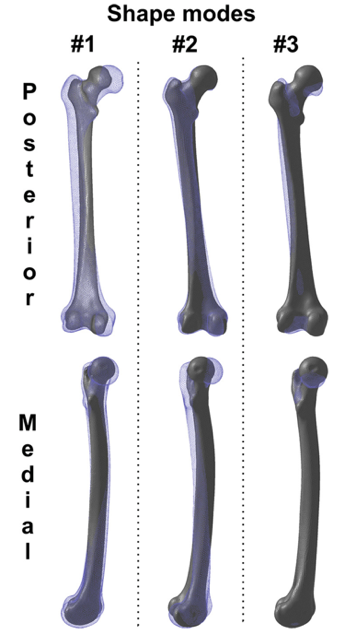
\includegraphics[width=2.30233in,height=4.23373in]{images/femurShape.png}
  \caption{Femoral shape
variations for the first three modes from the PCA. From 115 bones the
maximum eigenvalue is shown with the minimum eigenvalue shown in
wireframe. Taken from \cite{Grassi2014}.}
\label{fig:femur}
\end{figure}


In a study by Fitzpatrick et al. \cite{Fitzpatrick2011} statistical shape
models were
developed in order to identify the relationship between the shape and
function of the palletofemoral joint. Here, 26 magnetic resonance scans
of the knee were taken, from which FE models of the joint in question
were created. PCA was applied to the set of models, from which the first
15 principal components describing the shape were taken, these 15
components accounted for 97.2\% of the total geometric variation, with
the first component (PC1) counting for 47.7 \%. PC1, as is often the
case in biological models, described the variation in the size of the
joint components, with the next two components describing the position
of the patella and details regarding the conformity and depth of the
joint. Following modes of variation described more subtle variations in
the geometry of the model.

In order to assess the robustness or ability to accurately predict
outcomes of the reconstructed bones or joints, the studies
\cite{Grassi2014,Fitzpatrick2011} use a leave-one-out approach. This
approach
neglects one specimen from the development of the shape-function models.
The final model, based on the included specimens can be used to predict
the mechanics or properties of the left out specimen by using the
generated FE models.

\subsection{Discussion}\label{discussion}

The studies described above present useful workflows of generating
virtual subjects from a statistical model acquired from a databases of
scans. Such methods allow a variety of population based studies,
including those regarding the variation of vertebrae across the
population.

The ability to generate models not present in the input dataset and
hence create a large set of models representing the population allows us
to identify relationships not openly visible. For example in the study
by Fitzpatrick et al. \cite{Fitzpatrick2011} a 5 mm change in the patella
position
caused a 25\% increase in the contact pressure mid-flexion. This
relatively easy quantification of the relationship between geometry and
function can easily be transformed to quantify the relationship between
vertebral geometry and the mechanical response to vertebroplasty.
Equally, such relationships could enable the prediction of vertebral
fracture, adjacent level fracture or advise clinicians as to the
quantity and location of cement for different patients.


\section{Conclusion}

Vertebroplasty potentially provides a valuable method to treat patients with osteoporotic compression fractures, however, the uncertainty regarding its effects, especially regarding certain subsets of patients, mean that further research is required. While the mechanisms of pain relief are not fully understood, certain assumptions regarding the mechanical stabilisation and restoration of stiffness can be investigated. Such investigations may help to understand how patient groups respond to the
treatment in different ways.

Current experimental studies have provided a range of useful techniques for mechanically testing vertebrae and for carrying out the vertebroplasty procedure itself. However, obtaining enough vertebrae to represent variation across a population in order understand its effects on different patients is a difficult task and has not been attempted. A possible solution is FE modelling in conjunction with PCA. FE models have been shown to represent the intact vertebrae accurately using both $\mu$FE and continuum level models.

Problems arise when modelling the augmented vertebrae, with few studies modelling specimen specific augmented vertebrae and instead modelling vertebrae with arbitrary volumes of cement. Studies that have modelled and validated against experimental results have shown poor agreement, owing to the incorrect modelling of the cement-bone interface or incorrect selection of material properties for the cement-bone interdigitated region.

Finally, principal component analysis has shown its value in the literature presented above allowing the variation in a set of specimens to be accurately described and in certain cases models have been spawned at standard variations away from the mean.

\section{Aims \& Objectives}

The main aim for the project is to examine whether the outcomes for patients undergoing vertebroplasty are due to underlying biomechanical difference in their vertebrae. To achieve this overall aim three objectives have been defined:
\begin{enumerate}
\item To model specimen specific vertebrae accurately, initially using bovine tail vertebrae and later human vertebrae.
\item To carry out vertebra augmentation experimentally and accurately model the results of this augmentation in specimen specific models. This will require an investigation into the cement-bone interface within FE models, allowing the accurate modelling of augmented vertebrae.
\item To use PCA to identify patient subsets that respond differently to the mechanical outcomes of vertebroplasty.

\end{enumerate}

The first objective will require both experimental and computational work-flows.
Experimental work will focus on testing methods using bovine tail vertebrae, with an aim to adapt methods to use human vertebrae.
Computational work will concentrate on the creation of models of the bovine vertebrae that agree with experimental results for stiffness.

The second objective will involve developing methods of carrying out vertebroplasty on bovine specimens, aiming for clinically relevant volumes of cement using methods similar to those used in a clinical setting.
The computational side to this objective is to further the understanding of modelling cement-bone interfaces, allowing accurate models of augmented vertebrae to be made.

To achieve the final objective, an understanding of PCA will need to be developed along with how to apply it to vertebrae.
This will include methods of registering the volumes that define the vertebral body, applying the PCA algorithm and producing spawned vertebrae to help understand the variation in vertebrae of the population.

\pagebreak
